\documentclass{article}
\usepackage{fullpage}
\usepackage{amsfonts}
\usepackage{amsmath}
\usepackage{relsize}
\usepackage{tikz}
\usepackage{pgfplots}
\begin{document}
	\title{Edexcel AS and A Level Modular Mathematics\\ Core 3}
	\author{Elliott Whyman}
	\maketitle		
	\tableofcontents
	\section{Algebraic Fractions}
	\newpage
	\section{Functions}
	\subsection{Function Definition}
	A function is a mapping such that every element of set $A$ is mapped to exactly one element of set $B$.
	\\  
	The mapping set is considered to be the domain of the function, and the mapped set is considered to be the range.
	\\\\
	Consider the set, $A$, $\{1,2,3,4,5\}$ being mapped to set $B$, $\{1,4,16,25\}$ through the operation of $square$.
	Set $A$ is the domain and set $B$ is the range.
	\\\\
	The function can be defined by:
	\\\\
	\hspace*{\fill}{$f(x)=x^2$, $\{1\leq x \leq5\}$} \hfill {$f:x \rightarrow x^2$, $\{1\leq x \leq5\}$} \hspace*{\fill}
	\\\\
	\begin{center}
		It's range is subsequently defined by $$1\leq f(x) \leq 25$$
	\end{center}
	Consider the function $f:x \rightarrow \sqrt{x}$. It can only be considered a function if it's domain is greater than zero. Else it would have values less than zero that are not mapped anywhere as they do not have a real solution.
	\begin{center}
		$f:x \rightarrow \sqrt{x}$, $\{x \in \mathbb{R} , x \geq 0\}$
	\end{center}
	\subsection{Composite Functions}
	Multiple functions can be combined to make a composite function.
	\\\\
	\begin{center}
		\begin{tabular}{ccc}
			$fg(x)$ & $\Rightarrow$ & $f(g(x))$ \\
			$gf(x)$ & $\Rightarrow$ & $g(f(x))$ \\
			$f^2(x)$ & $\Rightarrow$ & $f(f(x))$
		\end{tabular}
	\end{center}
	To solve these composite functions, take the inner most function and input it as an parameter into the its nested function and so on.
	\subsection{Inverse Functions} \label{subsec:inverse}
	The inverse function performs the opposite operation in reverse order to get the original input of the function. When graphed, the inverse function is a reflection of the original function in the line $y=x$
	\\\\
	An inverse function is noted by $f^{-1}(x)$
	\\\\
	\begin{center}
		\begin{tabular}{rcl}
			$f(x)=x^2$ & $\Rightarrow$ & $f^{-1}(x)=\sqrt{x}$ \\
			$f(x)=5x+2$ & $\Rightarrow$ & $\displaystyle{ f^{-1}(x)=\frac{x-2}{5}}$ \\
			$f(x)=2x^2-9$ & $\Rightarrow$ & $\displaystyle{f^{-1}(x)=\sqrt{\frac{x+9}{2}}}$
		\end{tabular}
	\end{center}
	\newpage
	\section{Exponentials and Logarithmic Functions}
	Exponential functions are in the form $y=a^x$ and categories any functions containing exponents. 
	\subsection{The Exponential Function}
	The exponential function is $y=e^x$, $e \approx 2.718$. At any point, the function is equal to it's gradient, and is therefore refereed to as \textbf{the} exponential function. It is used to represent exponential growth, which is how population growth is modeled 
	\begin{center}
		$$\frac{d\lbrack e^x \rbrack}{dy}=e^x$$ 
	\end{center}
	\subsection{Graphing Exponential Functions}
	\begin{center}
		\begin{tikzpicture}
			\begin{axis}[axis lines = middle, xlabel = $x$, ylabel = $y$,]
				\addplot[domain=-2:2, color=red,]{exp(x)};
				\addlegendentry{$e^x$}
				\addplot[domain=-2:2, color=blue,]{exp(-x)};
				\addlegendentry{$e^{-x}$}
			\end{axis}
		\end{tikzpicture}
	\end{center}
	\subsection{The Inverse of the Exponential Function}
	To understand the inverse of the exponential function, it is necessary to read section \ref{subsec:inverse}.
	\\\\
	The inverse of $e^x$ is $\log_ex$. A log with base $e$ is referred to as the \textit{natural log}, $\ln x$. 
	
	\begin{center}
		\begin{tikzpicture}
		\begin{axis}[axis lines = middle, xlabel = $x$, ylabel = $y$, ymin=-5, ymax=5, samples=100, , xmin=-3]
		\addplot[domain=-5:5, color=red,]{exp(x)};
		\addlegendentry{$e^x$}
		\addplot[domain=-5:5,color=blue,]{ln(x)};
		\addlegendentry{$\ln x$}
		\addplot[domain=-5:5, color=black, dashed]{x};
		\end{axis}
		\end{tikzpicture}
	\end{center}
	\section{Numerical Methods}
	\subsection{Finding Approximations Graphically }
	\subsection{Finding Approximations Iteratively and Algebraically}
	\section{Transforming Graphs of Functions}
	\subsection{Sketching the Modulus Function}
	\subsection{Solving Equations Involving Modulus}
	\subsection{Applying Combinations of Transformations}
	\newpage
	\section{Trigonometry}
	\subsection{Introduction of Secant, Co-Secant and Co-Tangent Functions}
	\begin{center}
		\begin{tabular}{clcl}
			The Secant function is the reciprocal of the Sine function & $\sec\theta$ & = & $\displaystyle{\frac{1}{\cos\theta}}$ \\\\
			The Co-Secant function is the reciprocal of the Cosine function &$\csc\theta$ & = & $\displaystyle{\frac{1}{\sin\theta}}$ \\\\
			The Co-Tangent function is the reciprocal of the Sine Tangent function &$\cot\theta$ & = & $\displaystyle{\frac{1}{\tan\theta}}$ 
		\end{tabular}
	\end{center}
	An easy way to identify each function from its abbreviated notation is to compare its 3rd character to the begging of each standard Trigonometric Function
	\begin{center}
		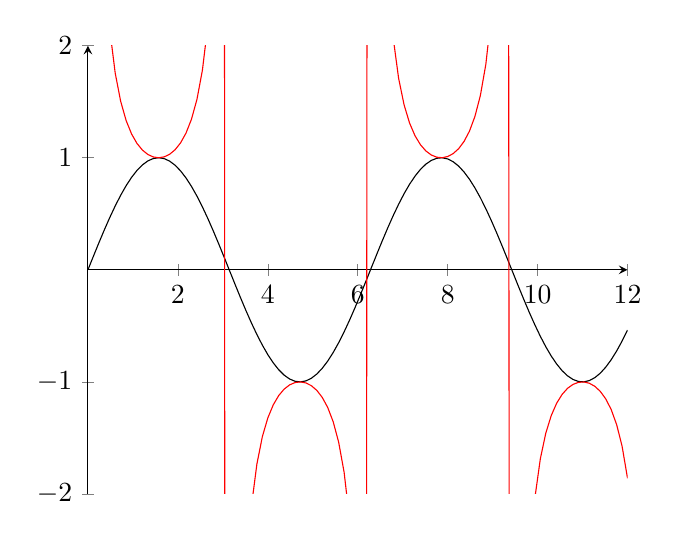
\begin{tikzpicture}
		\begin{axis}[axis lines = middle, domain=0:12, ymin=-2, ymax=2, xmin=0, xmax=12, samples=100]
			\addplot[color=black]{sin(deg(x))};
			\addplot[color=red]{cosec(deg(x))};
		\end{axis}
		\end{tikzpicture}
	\end{center}
	Above, the Sine function is graphed in black. As defined earlier it is that the Co-Secant function is reciprocal of the Sine function. \textit{Not to be confused with the inverse Sine function, $\arcsin$, $\sin^{-1}\theta$}. $$\csc\theta = \frac{1}{\sin\theta}$$ From analysing the plot above, asymptotes are present whenever the Sine function intersects with the x-axis, this is caused as at the intersection $\sin\theta=0$ and as $\csc\theta\equiv\frac{1}{\sin\theta}$ therefore $\csc\theta=\frac{1}{0}$ is undefined - causing an asymptote. This causes $y=\csc\theta$ to tend to infinity as it approaches  $\sin\theta=0$. $$\sin\theta \to 0 \Rightarrow \csc\theta\to\infty$$
	\\
	\begin{center}
		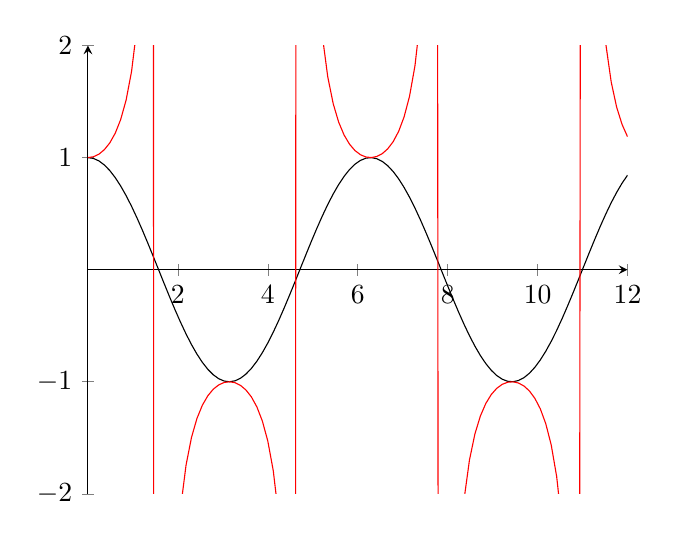
\begin{tikzpicture}
		\begin{axis}[axis lines = middle, domain=0:12, ymin=-2, ymax=2, xmin=0, xmax=12, samples=100]
		\addplot[color=black]{cos(deg(x))};
		\addplot[color=red]{sec(deg(x))};
		\end{axis}
		\end{tikzpicture}
	\end{center}
	The Cosine function above is also graphed in black, and we know it to be a transformation of the Sine function. As defined earlier it is that the Secant function is reciprocal of the Cosine function. \textit{Not to be confused with the inverse Cosine function, $\arccos$, $\cos^{-1}\theta)$}. $$\sec\theta = \frac{1}{\cos\theta}$$  From analysing the plot above, asymptotes are present whenever the Cosine function intersects with the x-axis, this is caused as at the intersection $\cos\theta=0$ and as $\sec\theta\equiv\frac{1}{\cos\theta}$ therefore $\sec\theta=\frac{1}{0}$ is undefined - causing an asymptote. This causes $y=\sec\theta$ to tend to infinity as it approaches $\cos\theta=0$. $$\cos\theta \to 0 \Rightarrow \sec\theta\to\infty$$
	\\
	\begin{center}
		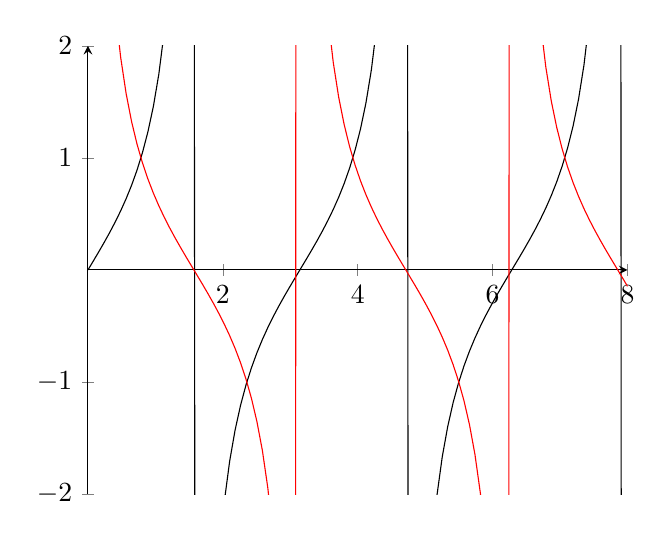
\begin{tikzpicture}
		\begin{axis}[axis lines = middle, domain=0:8, ymin=-2, ymax=2, xmin=0, xmax=8, samples=100]
		\addplot[color=black]{tan(deg(x))};
		\addplot[color=red]{cot(deg(x))};
		\end{axis}
		\end{tikzpicture}
	\end{center}
	Above, the Tangent function is graphed in black. As defined earlier it is that the Co-Tangent function is reciprocal of the Tan function. \textit{Not to be confused with the inverse Tangent function, $\arctan$, $\tan^{-1}(x)$}. $$\cot\theta = \frac{1}{\tan\theta}$$ From analysing the plot above, asymptotes are present whenever the Tan function intersects with the x-axis, as graphed on the normal Tangent function. As like before, there are also asymptotes whenever the Tangent function intersecs with the x-axis, this is caused as at the intersection $\tan\theta=0$ and as $\cot\theta\equiv\frac{1}{\tan\theta}$ therefore $\cot\theta=\frac{1}{0}$ is undefined - causing an asymptote. This causes $y=\cot\theta$ to tend to infinity as it approaches $\tan\theta=0$. $$\tan\theta \to 0 \Rightarrow \cot\theta\to\infty$$
	
	
	\subsection{Proving Identities}
	\section{Further Trigonometric Identities }
	\subsection{Addition Trigonometrical Formulae}
	\subsection{Double Angle Trigonometrical Formulae}
	\subsection{Expressing $a\cos\theta + b\sin\theta$ In a Single Trigonometric Function}
	\subsection{The Factor Fomulae}
	\section{Differentiation}
	\subsection{Differentiating Using The Chain Rule}
	\subsection{Differentiating Using The Product Rule}
	\subsection{Differentiating Using The Quotient Rule}
	\subsection{Differentiating The Exponential Function}
	\subsection{Differentiating The Logarithmic Function}
	\subsection{Differentiating The Trigonometric and Further Trigonometric Functions}
	\subsection{Differentiating Composite Functions}
\end{document}